%% abtex2-modelo-slides.tex, v-1.0 gfabinhomat
%% Copyright 2012-2016 by abnTeX2 group at http://www.abntex.net.br/ 
%%
%% This work may be distributed and/or modified under the
%% conditions of the LaTeX Project Public License, either version 1.3
%% of this license or (at your option) any later version.
%% The latest version of this license is in
%%   http://www.latex-project.org/lppl.txt
%% and version 1.3 or later is part of all distributions of LaTeX
%% version 2005/12/01 or later.
%%
%% This work has the LPPL maintenance status `maintained'.
%% 
%% The Current Maintainer of this work is Fábio Rodrigues Silva, 
%% member of abnTeX2 team, led by Lauro César Araujo. 
%% Further information are available on 
%% http://www.abntex.net.br/
%%
%% This work consists of the files abntex2-modelo-slides.tex, 
%% abntex2-modelo-references.bib and abntex2-modelo-marca.pdf
%%
%% Modelo desenvolvido por Fábio Rodrigues Silva (gfabinhomat@gmail.com)
%% Mais informações podem ser obtidas no guia do usuário Beamer 
%% (http://linorg.usp.br/CTAN/macros/latex/contrib/beamer/doc/beameruserguide.pdf)
%% Informações rápidas podem ser acessadas em http://en.wikibooks.org/wiki/LaTeX/Presentations


% Apresentações em widescreen. Outros valores possíveis: 1610, 149, 54, 43 e 32.
% Por padrão, as apresentações são no formato 4:3 (sem o aspectratio).
\documentclass[aspectratio=169]{beamer}	 	

\usetheme{Pittsburgh}
\usecolortheme{default}
\usefonttheme[onlymath]{serif}			% para fontes matemáticas
% Enconte mais temas e cores em http://www.hartwork.org/beamer-theme-matrix/ 
% Veja também http://deic.uab.es/~iblanes/beamer_gallery/index.html

% Customizações de Cores: fg significa cor do texto e bg é cor do fundo
\setbeamercolor{normal text}{fg=black}
\setbeamercolor{alerted text}{fg=red}
\setbeamercolor{author}{fg=blue}
\setbeamercolor{institute}{fg=blue}
\setbeamercolor{date}{fg=green}
\setbeamercolor{frametitle}{fg=red}
\setbeamercolor{framesubtitle}{fg=brown}
\setbeamercolor{block title}{bg=blue, fg=white}		%Cor do título
\setbeamercolor{block body}{bg=gray, fg=darkgray}	%Cor do texto (bg= fundo; fg=texto)

% ---
% PACOTES
% ---
\usepackage[alf]{abntex2cite}		% Citações padrão ABNT
\usepackage[brazil]{babel}		% Idioma do documento
\usepackage{color}			% Controle das cores
\usepackage[T1]{fontenc}		% Selecao de codigos de fonte.
\usepackage{graphicx}			% Inclusão de gráficos
\usepackage[utf8]{inputenc}		% Codificacao do documento (conversão automática dos acentos)
\usepackage{txfonts}			% Fontes virtuais
% ---

% --- Informações do documento ---
\title{Comparação entre algoritmos serial e paralelo escrito em C,
Java e Python}
\author{Taylan Branco Meurer \\ Leandro Loffi}
\institute{Programação Paralela e Multicore
	    \par
	    7º fase BCC}
\date{\today, v-1.9.6}
% ---

% ----------------- INÍCIO DO DOCUMENTO --------------------------------------
\begin{document}

% ----------------- NOVO SLIDE --------------------------------
\begin{frame}

\begin{minipage}{1\linewidth}
  \centering
  \begin{tabular}{cc}
    \begin{tabular}{c}
      
\includegraphics[width=3.0cm]{pictures/logo.jpg}
    \end{tabular}
    &
    \begin{tabular}{c}
      \textbf{Instituto Federal Catarinense} \\ \textbf{Campus Rio do Sul}
    \end{tabular}
  \end{tabular}
\end{minipage}

\titlepage

\end{frame}

% ----------------- NOVO SLIDE --------------------------------
\begin{frame}{Sumário}
\tableofcontents
\end{frame}

% ----------------- NOVO SLIDE --------------------------------
\section{Introdução}

\begin{frame}{Introdução}

Neste trabalho compara-se o desempenho de algoritmos seriais e paralelos. Os algoritmos realizam uma multiplicação entre matrizes quadradas e serão escritos em C, Java e Python. O paralelismo foi efetuado através da biblioteca OpenMP, do Jomp, do Multiprocessing e da linguagem Cython. Os tempos de execução foram obtidos por meio do comando time de um terminal bash. A métrica utilizada é baseada na Lei de Amdhal, portanto a linguagem com melhor desempenho em paralelo tem o maior speedup. Os algoritmos foram executados em uma máquina com Intel Core I7-3630QM, com SSD (mSATA) e com Sistema Operacional Debian stretch e Gnome 3.20.

\end{frame}

% ----------------- NOVO SLIDE --------------------------------
\section{OpenMP}
\begin{frame}
\frametitle{Diretivas OpenMP}
\framesubtitle{Diretivas utilizadas nos códigos paralelos}

\begin{block}{For}
  \#pragma omp for\\
  \#pragma omp for shared(A, B, C, size) private(i,j, k) num\underline{\hspace{.10in}}threads(8)
\end{block}

\begin{itemize}
 \item O primeiro for foi empregado na geração da matriz para o código C e Java\pause
 
 \item O segundo for foi empregado no procedimento que efetua a multiplicação entre matrizes \pause
 
 \item Para mais informações, consulte 
 \url{http://openmp.org/wp/}
 
\end{itemize}

\end{frame}

% ----------------- NOVO SLIDE --------------------------------
\begin{frame}{Multiprocessing}
\section{Multiprocessing}
Visite \url{https://docs.python.org/2/library/multiprocessing.html}.\\ 
Use-a como um guia de orientações gerais.
\vspace{0.7cm}

Multiprocessing é um módulo Python para processamento paralelo. Ele faz uso de uma API semelhante ao threading. 
O pacote multiprocessing oferece concorrência local e remota, contornando o Global Interpreter Lock através de subprocessos no lugar de threads. Por essa razão, esse módulo permite ao programador tirar proveito total dos múltiplos processadores em uma determinada máquina.

Visualizar código no repositório:
\begin{enumerate}
 \item \url{https://github.com/targueriano/MxM/blob/master/PyMxM_multiprocessing/pymxm_multiprocessing.py}
\end{enumerate}

\end{frame}

% ----------------- NOVO SLIDE --------------------------------
\begin{frame}{Cython}
\section{Cython}

Visite \url{http://docs.cython.org/src/userguide/parallelism.html}.\\ 
Use-a como um guia de orientações gerais.
\vspace{0.7cm}

O Cython pode ser definido como uma linguagem com tipos de dados em C. Quase todo código em Python é válido em Cython. Ele é uma linguagem que permite a geração de código C compilável e a geração de módulos para Python, tudo a partir de um código em Python. 

Visualizar código no repositório:
\begin{enumerate}
 \item \url{https://github.com/targueriano/MxM/blob/master/PyMxM_paralelo/pymxm_p.pyx}
\end{enumerate}


\end{frame}

% ----------------- NOVO SLIDE --------------------------------
\begin{frame}{Metodologia}
\section{Metodologia}

A metodologia faz uso da linguagem C, Java e Python (versão 2.7). Cada linguagem é composta por dois algoritmos, um serial e outro paralelo. O código paralelo em C é implementado com uso da API OpenMP. Em Java, o paralelismo é feito com Jomp e em Python com multiprocessing e Cython. 
O algoritmo implementa uma multiplicação entre matrizes. Essa implementação é bastante conhecida e generalista. Além disso, exige grande esforço computacional.

Os testes foram executados em uma máquina Intel Core I7 3630QM, CPU 3.4 GHz. A máquina possui 8GB de memória RAM e faz uso de um SSD mSATA. O Sistema Operacional instalado é o Debian stretch com kernel 4.6.0-1-amd64 e Gnome.

\end{frame}


% ----------------- NOVO SLIDE --------------------------------
\section{Resultados}

\begin{frame}{Resultados}
\frametitle{Tabela}
\framesubtitle{I}

\begin{table}[H]
  \centering
  \caption{Tempo de execução -- Java}
  \begin{tabular}{ccc}
    \hline
    Matriz(ordem) & Serial(s) & Paralelo(s) -- Jomp\\
    \hline
    \hline
    500 & 0.228 & 0.189\\
    1000 & 0.845 & 0.413\\
    1500 & 2.590 & 1.000\\
    2000 & 6.274 & 2.157\\
    \hline
  \end{tabular}
  \label{tab:timeJava}
\end{table}

\end{frame}

% ----------------- NOVO SLIDE --------------------------------
\begin{frame}{Resultados}
\frametitle{Tabela}
\framesubtitle{II}

\begin{table}[H]
  \centering
  \caption{Tempo de execução -- C}
  \begin{tabular}{ccc}
    \hline
    Matriz(ordem) & Serial(s) & Paralelo(s)\\
    \hline
    \hline
    500 & 0.446 & 0.127\\
    1000 & 3.292 & 0.898\\
    1500 & 11.461 & 3.189\\
    2000 & 26.847 & 7.235\\
    \hline
  \end{tabular}
  \label{tab:timec}
\end{table}

\end{frame}

% ----------------- NOVO SLIDE --------------------------------
\begin{frame}{Resultados}
\frametitle{Tabela}
\framesubtitle{III}

\begin{table}[H]
  \centering
  \caption{Tempo de execução -- Cython}
  \begin{tabular}{ccc}
    \hline
    Matriz(ordem) & Serial(s) & Paralelo(s) -- Cython \\
    \hline
    \hline
    500 & 0.837 &  0.504 \\
    1000 & 10.186 & 3.841\\
    1500 & 30.911 & 12.314\\
    2000 & 1min41.794 & 29.442\\
    \hline
  \end{tabular}
  \label{tab:timePy1}
\end{table}

\end{frame}

% ----------------- NOVO SLIDE --------------------------------
\begin{frame}{Resultados}
\frametitle{Tabela}
\framesubtitle{IV}

\begin{table}[H]
  \centering
  \caption{Tempo de execução -- Python2.7}
  \begin{tabular}{ccc}
    \hline
    Matriz(ordem) & Serial(s) & Paralelo(s) -- Multiprocessing \\
    \hline
    \hline
    500 & 1.021 &  0.912 \\
    1000 & 17.073 & 9.797\\
    1500 & 1min7.847 & 31.116\\
    2000 & 2min27.214 & 1min17.700\\
    \hline
  \end{tabular}
  \label{tab:timePy2}
\end{table}

\end{frame}



% ----------------- NOVO SLIDE --------------------------------
\begin{frame}
\frametitle{Gráficos}
\framesubtitle{I}

\begin{figure}
  \centering
  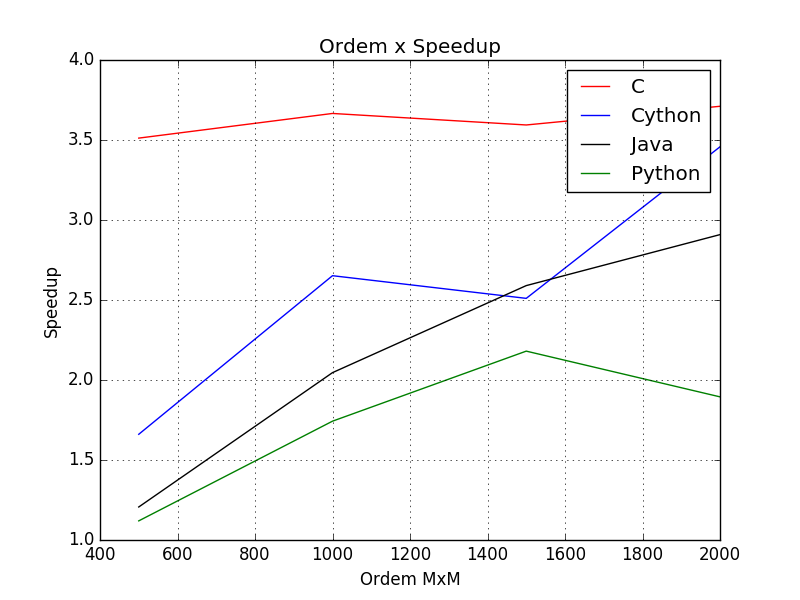
\includegraphics[width=8cm]{pictures/speedup_full2.png}
  \caption{Speedup {\small Fonte: do autor}}
\end{figure}

\end{frame}

% ----------------- NOVO SLIDE --------------------------------
\begin{frame}{Resultados}
\frametitle{Gráficos}
\framesubtitle{II}

\begin{figure}
  \centering
  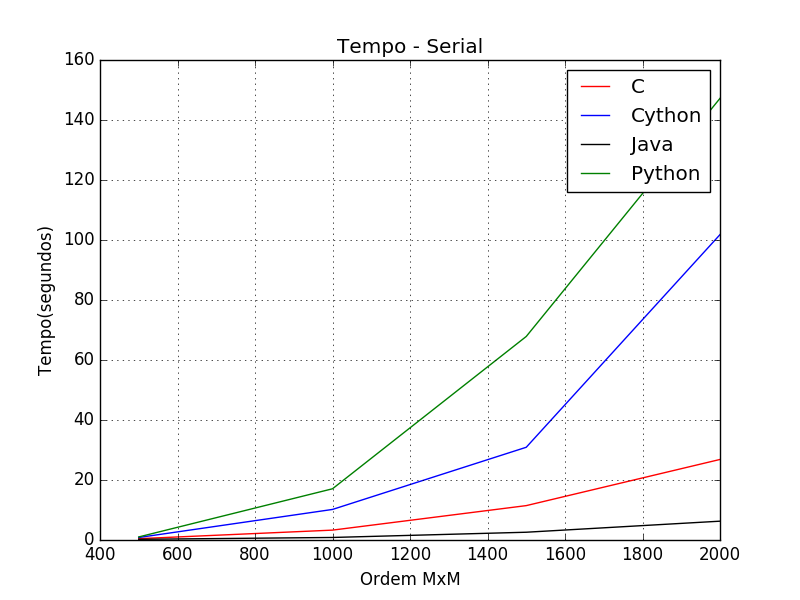
\includegraphics[width=8cm]{pictures/tempo_serial.png}
  \caption{Tempo serial {\small Fonte: do autor}}
\end{figure}

\end{frame}

% ----------------- NOVO SLIDE --------------------------------
\begin{frame}{Resultados}
\frametitle{Gráficos}
\framesubtitle{III}

\begin{figure}
  \centering
  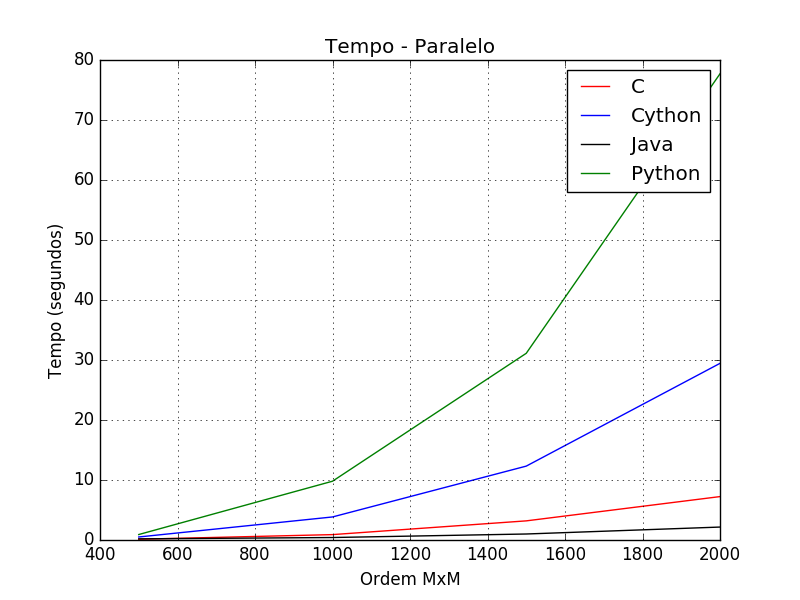
\includegraphics[width=8cm]{pictures/tempo_paralelo.png}
  \caption{Tempo paralelo {\small Fonte: do autor}}
\end{figure}

\end{frame}


% ----------------- NOVO SLIDE --------------------------------
\section{Conclusão}
\begin{frame}{Conclusão}

A partir dos resultados, que são bem limitados, nota-se que o emprego do OpenMP é mais vantajoso para a linguagem nativa, a saber, a C. Embora haja diversos projetos, bibliotecas ou módulos eficientes para as linguagens apresentadas nesse artigo, a interação entre API e linguagem ainda não é madura suficiente.

\end{frame}



% ----------------- NOVO SLIDE --------------------------------
\section{Referências}

% --- O comando \allowframebreaks ---
% Se o conteúdo não se encaixa em um quadro, a opção allowframebreaks instrui 
% beamer para quebrá-lo automaticamente entre dois ou mais quadros,
% mantendo o frametitle do primeiro quadro (dado como argumento) e acrescentando 
% um número romano ou algo parecido na continuação.

\begin{frame}[allowframebreaks]{Referências}
\footnotesize
{
  \begin{thebibliography}{99} % Beamer does not support BibTeX so references must be inserted manually as below
  \bibitem[Chandra, 2001]{p1} CHANDRA, R. et al. (2001)
  \newblock “Parallel programming in openmp”
  \newblock \emph{Morgan Kaufmann}.


  \end{thebibliography}
}

\bibliography{abntex2-modelo-references}

\end{frame}

% ----------------- FIM DO DOCUMENTO -----------------------------------------
\end{document}
